\section{Theoretische Grundlage}
\label{sec:Theorie}

Ziel dieses Versuches ist es mit Hilfe verschiedener Brückenschaltungen unbekannte Widerstände, Kapazitäten und Induktivitäten auszumessen. Dies wird zum Beispiel mittels einer Abgleichbedingung realisiert.
Jede Brückenschaltung wird prinzipiell von einer Speisepannung $U_\text{s}$ und vier Widerständen betrieben, siehe Abbildung \ref{fig:wheatstone}. Dies kann auch durch Scheinwiderstände realisiert werden, was impliziert das die Brückenschaltung je nach Aufbau mit Wechselstrom betrieben werden muss.
\begin{figure}[H]
	\centering
	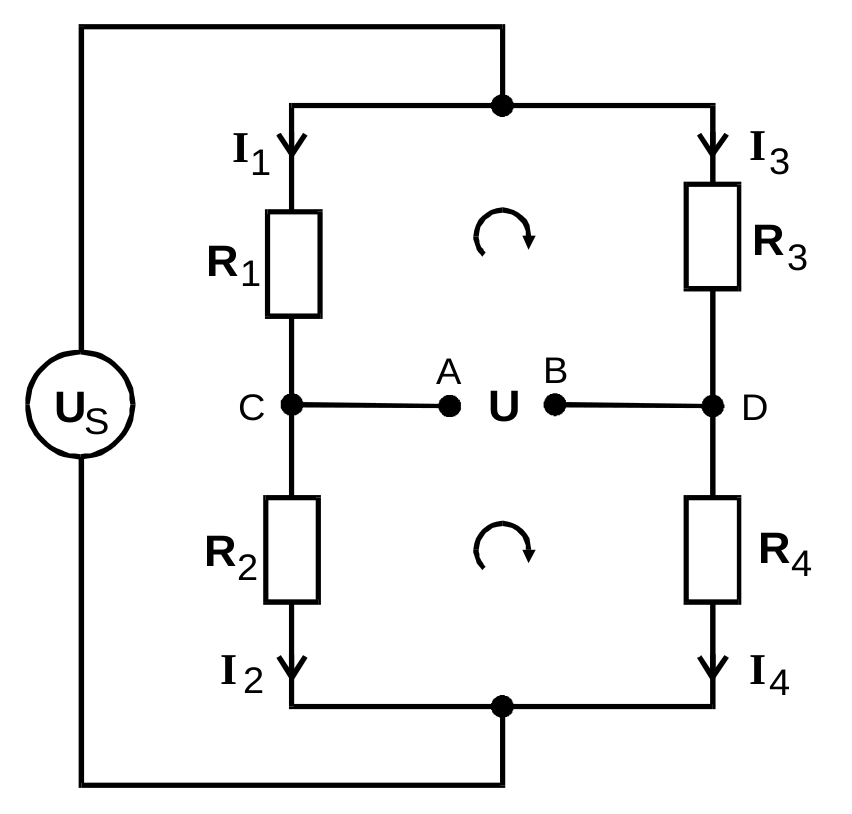
\includegraphics[height=5cm]{picture/1.png}
	\caption{Wesentlicher Aufbau einer Brückenschaltung \cite{sample}.}
	\label{fig:wheatstone}
\end{figure}
Die Brückenschaltung liegt dem Kirchhoffschen Regeln zu Grunde. Die erste der beiden Regeln besagt, dass die Summe der eingehenden und ausgehende Ströme an einem Knoten gleich Null ist.
\begin{equation}
  \text{Knotenregel} : \sum_{\text{k=1}}^\text{n} I_\text{k} = 0
  \label{eqn:K1}
\end{equation}
Die zweite Regel besagt, dass sich bei einer Geschlossenen Masche alle Teilspannungen, bei einem Umlauf zu Null addieren.
\begin{equation}
  \text{Maschenregel} : \sum_{\text{k=1}}^\text{n} U_\text{k} = 0 \ .
  \label{eqn:K2}
\end{equation}
Unter Berücksichtigung der Kirchhoffschen Gesetze ergibt sich für die einfachste Brückschaltung eine Brückenspannung $U_\text{Br}$ von
\begin{equation}
  U_\text{Br} = \frac{R_2 R_3 - R_1 R_4}{(R_3 + R_4)(R_1 + R_2)} \ .
  \label{eqn:Ubr}
\end{equation}
Es wird das Widerstandverhältnis so gewählt, dass die Brückenspannung minimal wird. Daraus ergibt sich die Abgleichsbedingung
\begin{equation}
  R_2 R_3 = R_1 R_4 \ .
  \label{eqn:R}
\end{equation}
Für komplexe Widerstände ändert sich die Abgleichsbedingung zu
\begin{align}
	\xi_1 \xi_4 & = \xi_2 \xi_3
	\label{eqn:XY}
\end{align}
\begin{align*}
		\text{mit} \ \xi & = X + iY \ .
\end{align*}
Da zwei komplexe Zahlen nur dann gleich sind, wenn sie in Real- und Imaginärteil übereinstimmen, lautet \ref{eqn:XY} ausführlich geschrieben
\begin{align}
	X_1 X_4 - Y_1 Y_4 = X_2 X_3 - Y_2 Y_3
	\label{eqn:XY1}
\end{align}
und
\begin{align}
	X_1 Y_4 + X_4 Y_1 = X_2 Y_3 + X_3 Y_2 \ .
	\label{eqn:XY2}
\end{align}

\subsection{Wheatston'sche Brückenschaltung}
Die Wheatstone Brücke besteht ausschließlich aus ohmschen Widerständen. Sie ist dafür gedacht einen unbekannten Widerstand $R_\text{x}$ mittels der oben genannten Abgleichmethode zu bestimmen. Der Schematische Aufbau einer Wheatstone Brücke ist in Abbildung \ref{fig:widerstand} zu sehen.
\begin{figure}[H]
      \centering
      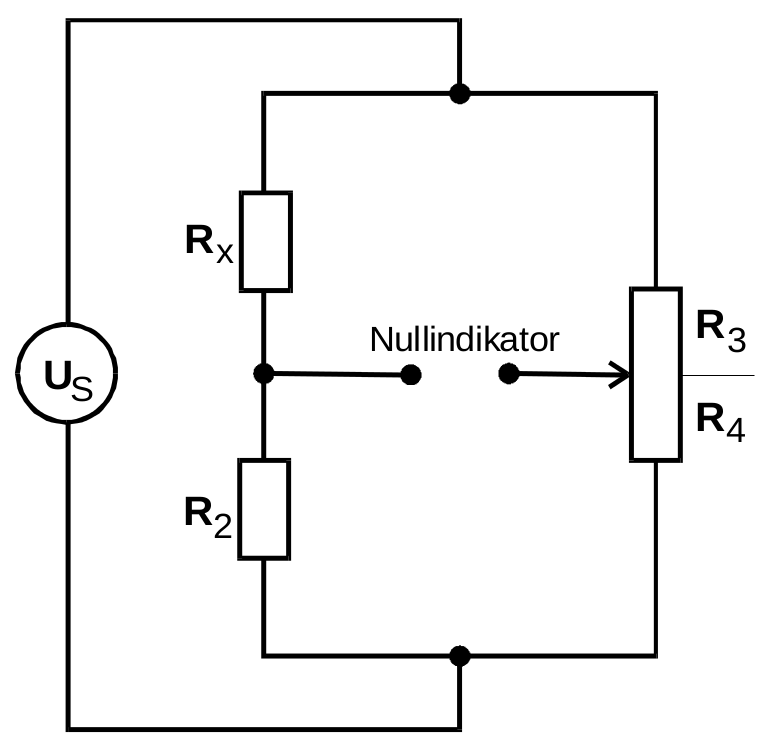
\includegraphics[height=5cm]{picture/2.png}
      \caption{Aufbau einer Wheatstone Brücke \cite{sample}.}
      \label{fig:widerstand}
\end{figure}
Der Widerstand $R_\text{x}$ ergibt sich aus dem Umstellen der Gleichung \ref{eqn:R} zu
\begin{equation}
  R_x = R_2 \frac{R_3}{R_4} \ .
  \label{eqn:R_x}
\end{equation}
Das Verhältniss $R_3$ zu $R_4$ lässt sich besonders gut mit Hilfe eines Potentiometer einstellen.
\subsection{Kapazitätsmessbrücke}
In Abbildung \ref{fig:C} ist der Aufbau einer Kapazitätsmessbrücke dargestellt, mit Hilfe der Kapazitätsmessbrücke soll die Kapazität des Kondensators bestimmt werden. Dies geschieht über die Impedanz des Kondensators, daher muss der Aufbau mit Wechselstrom betrieben werden. Da es sich im Versuch um keinen idealen Kondensator handelt wird im Schaltbild ein fiktiver Widerstand $R_\text{x}$ vor den Kondensator geschaltet.
\begin{figure}[H]
  \centering
  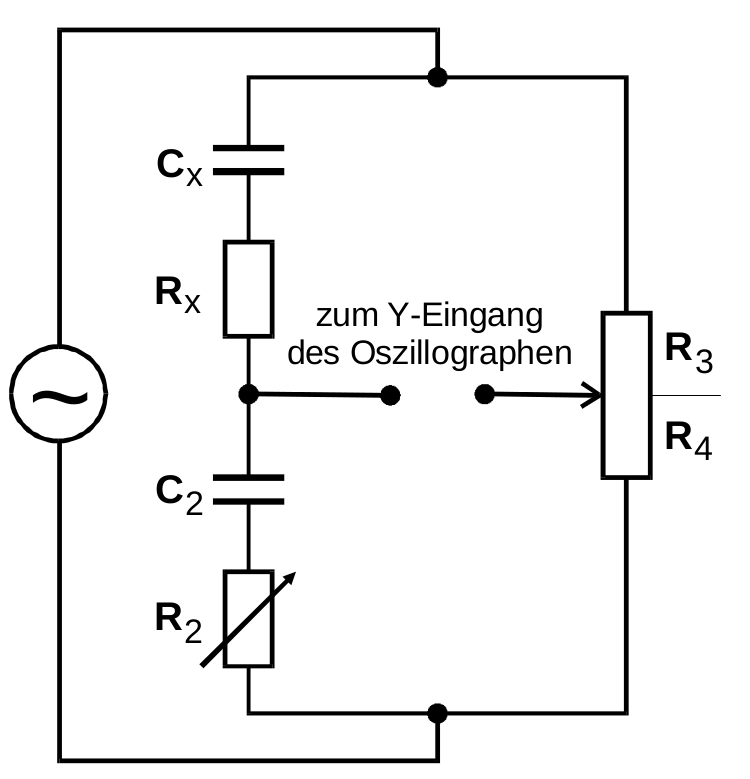
\includegraphics[height=5cm]{picture/3.png}
  \caption{Messung der Kapazität eines realen Kondensators \cite{sample}.}
  \label{fig:C}
\end{figure}
Mittels der Abgleichbedingung gibt sich analog zu Formel \ref{eqn:R_x} ein Widerstand von
\begin{equation*}
    R_\text{x} = R_2 \frac{R_3}{R_4} \ ,
\end{equation*}
und für die Kapazität des Kondensators unter Berücksichtigung der Scheinwiderstände nach GLeichung \ref{eqn:XY2} folgt
\begin{equation}
  C_\text{x} = C_2 \frac{R_4}{R_3} \ .
  \label{eqn:C_x}
\end{equation}

\subsection{Induktivitätsmessbrücke}
Mittels der Messbrücke aus der Abbildung \ref{fig:L} soll die Induktivität einer Spule bestimmt werden. Dies geschieht Analogie zur Kapazitätsmessbrücke über die Impedanz der Spule,daher muss der Aufbau mit Wechselstrom betrieben werden.

\begin{figure}[H]
  \centering
  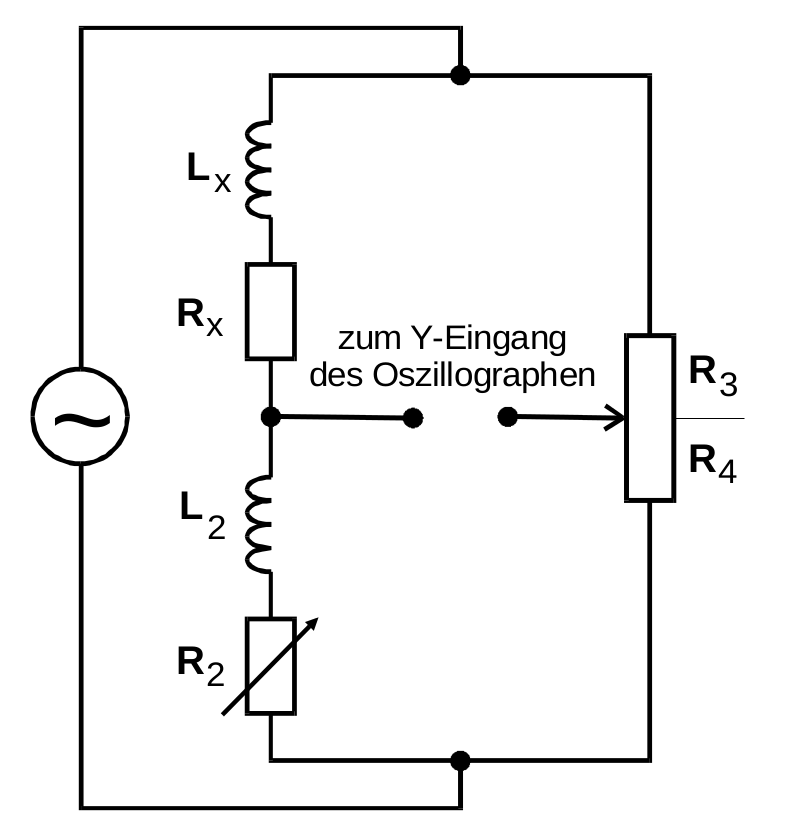
\includegraphics[height=5cm]{picture/4.png}
  \caption{Messung der Induktivität einer realen Spule \cite{sample}.}
  \label{fig:L}
\end{figure}
Mittels der Abgleichbedingung gibt sich analog zu Formel \ref{eqn:R_x} ein Widerstand von
\begin{equation*}
     R_\text{x} = R_2 \frac{R_3}{R_4} \ ,
\end{equation*}
und für die Induktivität der Spule unter Berücksichtigung der Scheinwiderstände nach GLeichung \ref{eqn:XY2} folgt
\begin{equation}
   L_\text{x} = L_2 \frac{R_3}{R_4} \ .
   \label{eqn:L_x}
\end{equation}
\subsection{Maxwell-Brücke}
Es soll die Induktivität einer Spule mit Hilfe der Maxwell-Brücke bestimmt werden. Dafür wird anstelle einer Spule, wie im vorherigen Kapitel beschrieben, ein Kondensator verwendet und wie in Abbildung \ref{fig:Max-Br} aufgebaut. Es muss darauf geachtet werden, dass einerseits, die Frequenz hoch genug ist, damit sich der Einschwingvorgang hinreichend schnell einstellt und andererseits die Frequenz niedrig genug ist, damit die Streukapazitäten niedrig genug sind um einen Abgleich zu ermöglichen.
\begin{figure}
  \centering
  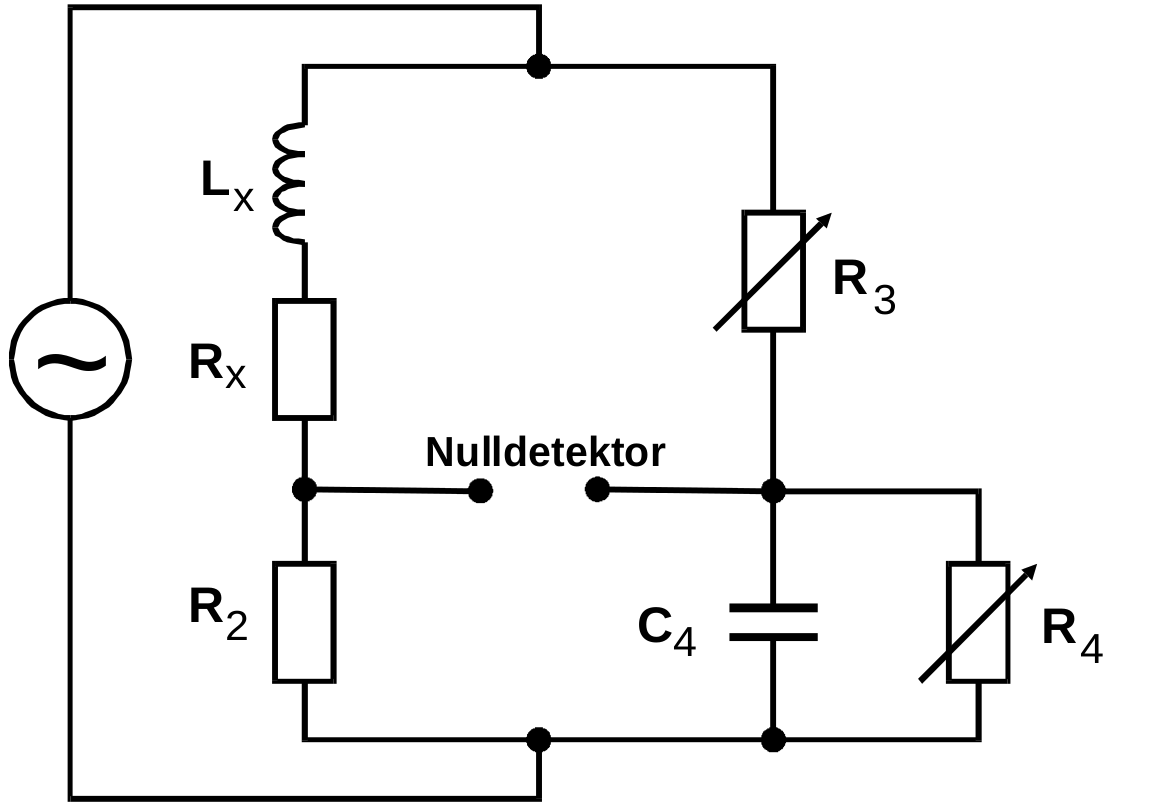
\includegraphics[height=5cm]{picture/5.png}
  \caption{Messung der Induktivität durch eine Maxwell-Brücke \cite{sample}.}
  \label{fig:Max-Br}
\end{figure}
Aus den Gleichungen \ref{eqn:XY1} und \ref{eqn:XY2} ergeben sich $L_\text{x}$ und $R_\text{x}$ zu
\begin{equation}
  L_\text{x} = R_2 R_3 C_4
  \label{eqn:L_m}
\end{equation}
und
\begin{equation*}
  R_\text{x} = R_2 \frac{R_3}{R_4} \ .
\end{equation*}

\subsection{TT-Brücke}
Mittels einer TT-Brücke soll die Funktion des elektrischen Filters genauer bestimmt werden. Dafür wird die Schaltung Abbildung \ref{fig:TT} entsprechend aufgebaut.
\begin{figure}
  \centering
  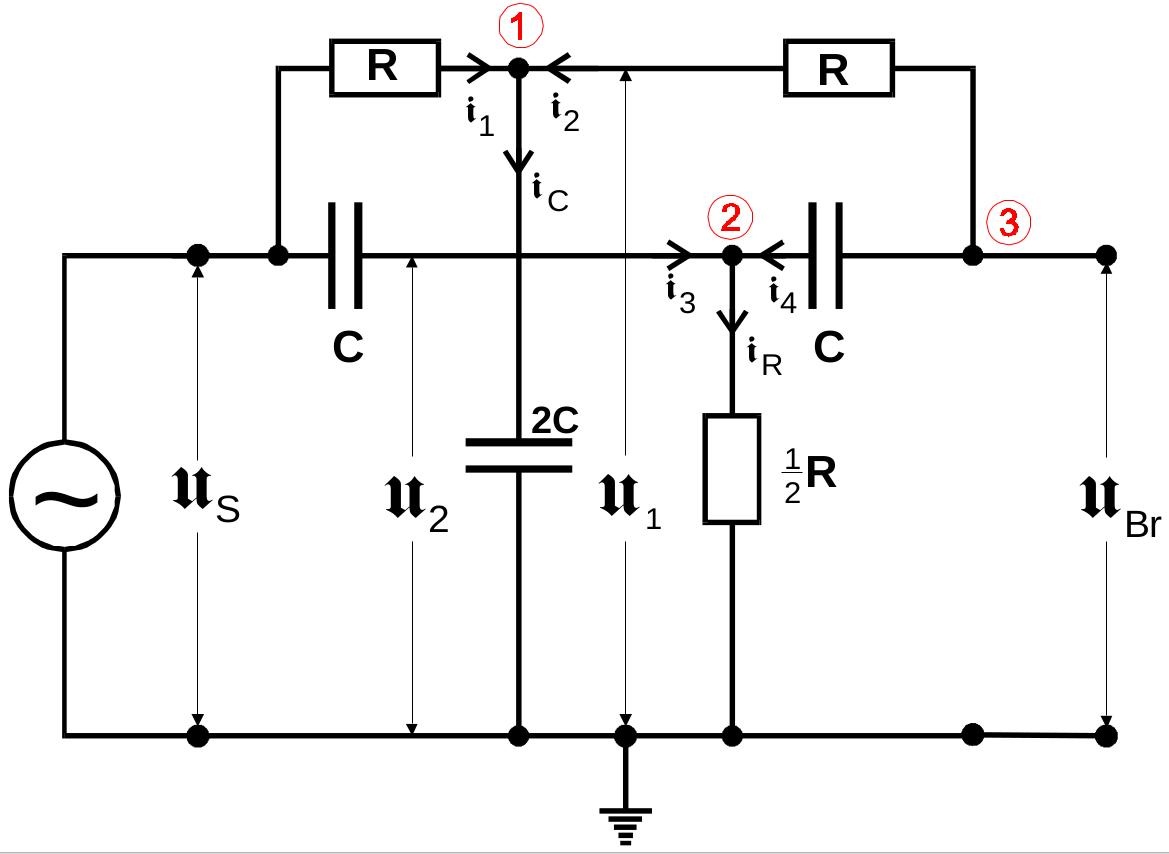
\includegraphics[height=5cm]{picture/7.png}
  \caption{Messung der Induktivität durch eine TT-Brücke \cite{sample}.}
  \label{fig:TT}
\end{figure}
Das Spannungverhältniss $U_\text{Br}$ zu $U_\text{S}$ zu berechnen werden die Ströme an den Knoten 1, 2 und 3 betrachtet. Für den ersten Knoten ergibt sich nach der Kirchhoffschen Knotenregel
\begin{equation}
  \frac{U_1 - U_\text{S}}{R} + \frac{U_1 - U_\text{Br}}{R} = 2 i \omega C U_1 \ .
  \label{eqn:M1}
\end{equation}
Mit Hilfe der Ströme an dem zweiten
\begin{equation}
  \left( U_\text{S} - U_2 \right) i \omega C + \left( U_\text{Br} - U_2 \right)i \omega C = \frac{2}{R} U_2
  \label{eqn:M2}
\end{equation}
und dritten Knoten
\begin{equation}
  \left( U_2 - U_\text{Br} \right)i \omega C + \frac{U_q - U_\text{Br}}{R} = 0
  \label{eqn:M3}
\end{equation}
lässt sich durch Auflösen der Gleichungen \ref{eqn:M1}, \ref{eqn:M2} nach $U_1$ und $U_2$ und deren Ergebnisse in \ref{eqn:M3} eingesetzt, die Brückenspannung ermitteln.
\begin{equation}
  U_\text{Br} = U_\text{S} \frac{1 - \omega^2 R^2 C^2}{1 - \omega^2 R^2 C^2 + 4 i \omega R C}
  \label{eqn:Ubr}
\end{equation}
Durch das Umstellen der Gleichung \ref{eqn:Ubr} und das Einführen von $\Omega$ folgt
\begin{equation*}
  \Omega = \omega R C \ ,
\end{equation*}
die Form
\begin{equation*}
  \frac{U_\text{Br}}{U_\text{S}} = \frac{1 - \Omega^2}{1 - \Omega^2 + 4 i \Omega} \ .
\end{equation*}
Hieraus erhält man durch Multiplikation mit dem konjugiert komplexen Wert
des Nenners den Ausdruck:
\begin{equation}
  \left| \frac{U_\text{Br}}{U_\text{S}} \right|^2 = \frac{(1 - \Omega^2)^2}{(1 - \Omega^2)^2 + 16 \cdot \Omega^2} \ .
  \label{eqn:BrS}
\end{equation}

\subsection{Fehlerrechnung}
\subsubsection{Mittelwert}
Der Mittelwert einer Messreihe $x_1, ... ,x_\text{n}$ lässt sich durch die Formel
\begin{equation}
	\overline{x} = \frac{1}{N} \sum_{\text{k}=1}^\text{N} x_k
	\label{eqn:ave}
\end{equation}
berechnen. Die Standardabweichung des Mittelwertes beträgt
\begin{equation}
	\Delta \overline{x} = \sqrt{ \frac{1}{N(N-1)} \sum_{\text{k}=1}^\text{N} (x_\text{k} - \overline{x})^2}
	\label{eqn:std}
\end{equation}

\subsubsection{Fehlerfortpflanzung mit Python}
Die Fehlerfortpflanzung wird im folgenden mit Hilfe von der Funktion "ufloat" aus "python-uncertainties" durchgeführt. Die dafür verwendete Versionsnummer von Python ist 3.4.3.
